%!TeX root = SM_Thesis_Proposal.tex

\section{Introduction}
\label{sec:introduction}

Many containerization systems rely on Linux's isolation primitives, exposed via
the cgroups interface, in order to enforce the isolation between different
containers.\ cgroups interface files allow for the control of resources,
including cpu, memory, and i/o. In this thesis we take a closer look at the way
the cpu isolation is used and enforced. 

Kubernetes\cite{kubernetes}, for example, allows users to specify cpu resource
requirements in two ways: requests and limits. Limits are directly passed on to
the cgroups cpu.limit interface. Linux implements cpu limits using accounting to
ensure that the processes in the cgroup get no more cpu time than
allowed.
% \hmng{do we care to explain the details?}

For Kubernetes' resource requests interface, it is desirable that containers be
allowed to burst when possible. For example, a service $s_1$ might ask for two
CPUs, but occasionally have bursts of load. If $s_1$ is on an otherwise empty
machine with more than two CPUs, or collocated with a different service that is
experiencing less load than usual, $s_1$ should be able to use more than its
requested two CPUs. In order to support this, Kubernetes relies on cgroups'
weight feature. Weights in cgroups allow for the desired bursting: the cpu time
processes should get is determined by the ratio of the process's weight ($w_p$)
to the weight of all \textit{runnable} processes ($W = \sum_i w_i$). For
example, suppose cgroup $cg_1$ is supposed to get one CPU and $cg_2$ three CPUs,
their weights would be set to have a 1:3 ratio. If both cgroups have enough load
to fill that capacity, then they are constantly in contention for resources and
the scheduler ensures that $cg_1$ is running $\frac{1}{3}$ of the time, and
$cg_2$ $\frac{2}{3}$ of the time, amounting to effectively $cg_1$ getting one
CPU and $cg_2$ three, as desired. However, if $cg_2$ has less load, there will
be times where it has no runnable threads on some of the cores, and on those
cores the threads in $cg_1$ will represent 100\% of the weight there and be able
to run uncontended.


\begin{figure*}[t]
    \centering
    \begin{subfigure}[t]{0.48\textwidth}
        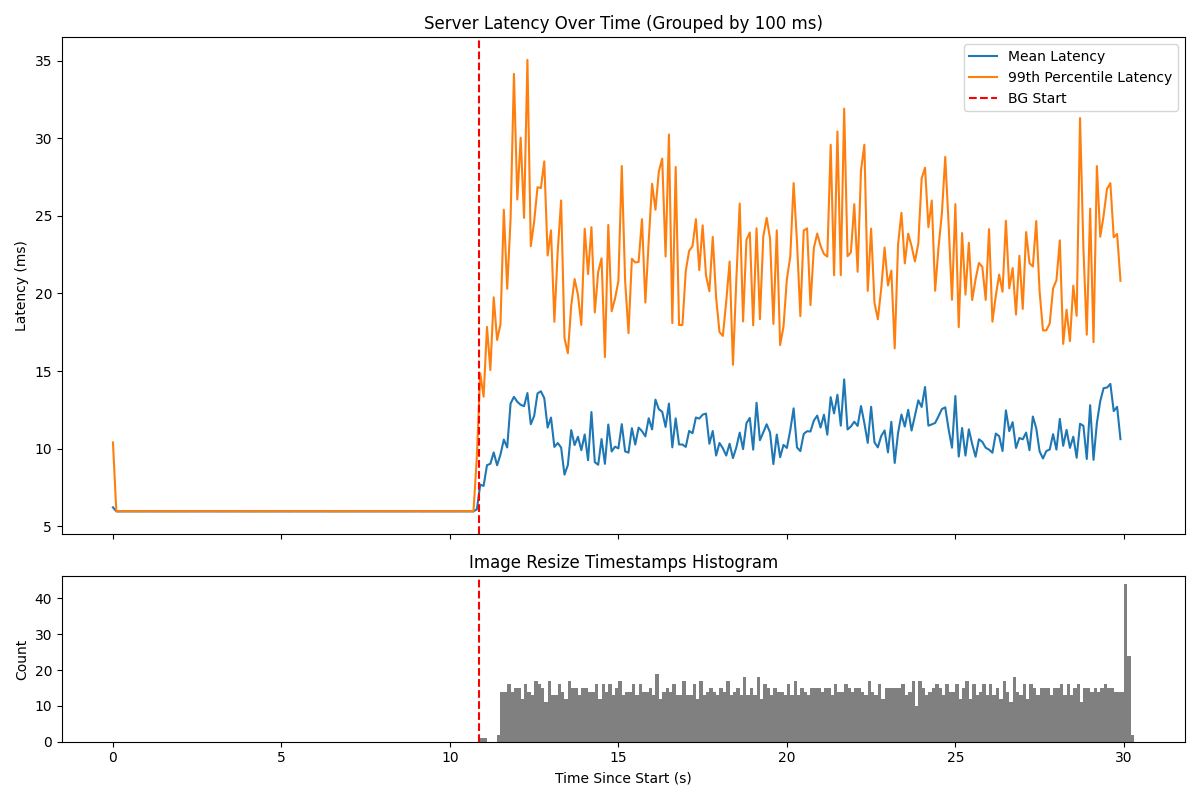
\includegraphics[width=\textwidth]{graphs/unedited-weight-low-two.png}
        \caption{Low load stetting}\label{fig:unedited-weight-low-two}
    \end{subfigure}
    \hspace{\fill}
    \begin{subfigure}[t]{0.48\textwidth}
        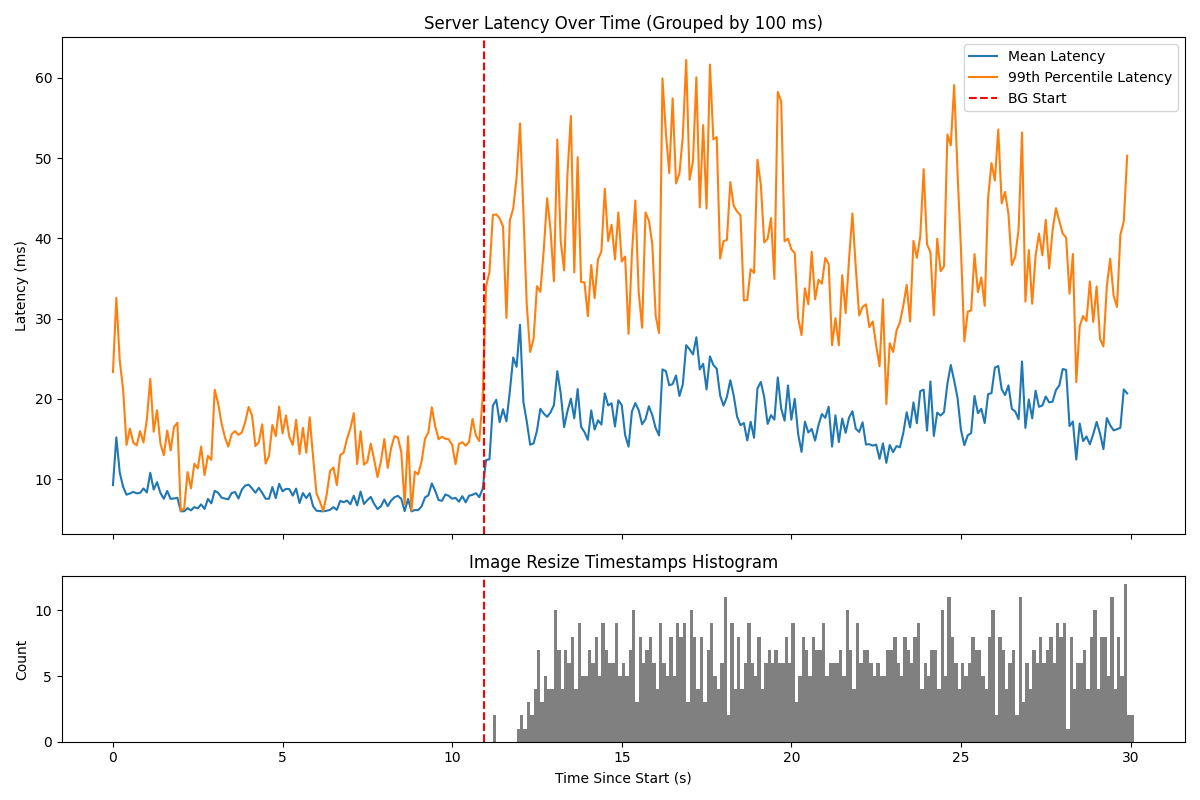
\includegraphics[width=\textwidth]{graphs/unedited-weight-high-two.png}
        \caption{High load setting}\label{fig:unedited-weight-high-two}
    \end{subfigure}
    \caption{Latencies of the server and iteration counts of the background
    tasks in different load scenarios. Note the different y axis limits. The
    upper graphs show end-to-end request latencies, and the bottom graph is a
    histogram of completed iterations of the BE tasks}
\end{figure*}

They way Kubernetes supports BE tasks is by setting containers without any CPU
requests to have the lowest weight possible.\ cgroups cpu.weight is clamped to
be between the values of 1 and 10,000, meaning BE tasks have weight 1. This is
in principle a large range, and should allow for BE tasks to have a negligible
performance impact on LC tasks, even during high load. 

However, we find that even when setting the weights of processes to the
outermost extremes, the presence of low weight (ie BE) tasks has a large
performance impact on a high-weight (ie LC) task. In an experiment, we run a
(LC) server that processes requests coming in from an open loop client, running
on a separate machine. The client has 100 connections to the server, each
connection creates a new server thread that reads from the socket and
synchronously processes requests in a tight loop. The server threads run in a
cgroup with the highest possible weight: 10000. The server initially runs on an
uncontended four cores, during which time the cpu utilization of the server is
around 85\%. After $\sim$10 seconds, we start two background tasks on the same
four cores, each performing an image resize job. Each background task is in its
own cgroup, which both have the lowest possible weight, 1. We then measure the
latencies experienced by the LC server, before and after starting the background
tasks. Figure~\ref{fig:unedited-weight-low-two} shows the results. We see that
mean latencies spike up from steady at just under 6ms to as high as 13ms, and
much higher for 99th percentile latencies.

With a higher baseline load for the LC server the spikes are higher,
figure~\ref{fig:unedited-weight-high-two} shows the latencies when the
utilization of the uncontended server load is around 95\%.







